% Standalone render of generated_intraday_dh/table_rule_by_strategy_dh_holdclose_pooled.tex
% Build: pdflatex -interaction=nonstopmode rule_by_strategy_dh_holdclose_pooled.tex
\documentclass{article}
\usepackage[landscape,margin=0.5in]{geometry}
\usepackage{booktabs}
\usepackage{amsmath}
\usepackage{graphicx}
\pagestyle{empty}

\begin{document}
\begin{center}
\textbf{0DTE nearest-OTM straddle: per-rule return summary, pooled over the twelve entry windows 10:00--15:30 ET (overlapping remaining-session books), models compared on the same 866 days}\\[1.5ex]
% AUTO-GENERATED by writeup/make_rule_by_strategy_intraday_tex.py -- do not edit.
% Source: results/atm_straddle_intraday/rule_by_strategy/pooled/rule_by_strategy_*.csv
\begingroup\small\setlength{\tabcolsep}{3.6pt}
\begin{tabular}{lrrrrrrrrrrrr}
\toprule
& $n$ & mean & std & min & max & skew & ex.\ kurt & $t$ & Sharpe$_{\mathrm{ann}}$ & $n_{\mathrm{buy}}$ & \%buy & Sharpe$^{\times}_{\mathrm{ann}}$ \\
\midrule
\multicolumn{13}{l}{\emph{Short volatility (always short)}} \\
all models (no forecast) & 866 & 1.014 & 5.487 & -54.71 & 10.01 & -2.40 & 14.95 & 5.44 & 2.93 & 0 & 0.0 & 2.21 \\
\midrule
\multicolumn{13}{l}{\emph{$\mathrm{sign}(s)$ ($\pm 1$ on the sign of $s$)}} \\
baseline (HAR + calendar OLS) & 866 & 0.446 & 3.633 & -16.36 & 48.77 & 2.45 & 36.72 & 3.61 & 1.95 & 266 & 30.7 & 0.86 \\
block-diagonal ridge & 866 & 0.560 & 3.727 & -20.53 & 54.71 & 3.21 & 52.60 & 4.42 & 2.38 & 252 & 29.1 & 1.33 \\
block-diagonal ridge, without the FOMC columns & 866 & 0.532 & 3.690 & -16.36 & 54.71 & 3.55 & 53.83 & 4.25 & 2.29 & 267 & 30.8 & 1.22 \\
LightGBM$^{\dagger}$ & 866 & 0.536 & 3.725 & -20.53 & 54.71 & 3.32 & 52.85 & 4.23 & 2.28 & 277 & 32.0 & 1.23 \\
XGBoost$^{\dagger}$ & 866 & 0.524 & 3.738 & -20.53 & 54.71 & 3.30 & 52.17 & 4.13 & 2.23 & 271 & 31.3 & 1.17 \\
lasso (causally tuned)$^{\dagger}$ & 866 & 0.494 & 3.658 & -20.53 & 48.77 & 2.36 & 36.43 & 3.98 & 2.14 & 276 & 31.9 & 1.07 \\
lasso ($\alpha=10^{-4}$) & 866 & 0.561 & 3.491 & -20.53 & 37.84 & 1.00 & 16.98 & 4.73 & 2.55 & 248 & 28.6 & 1.42 \\
elastic net (causally tuned)$^{\dagger}$ & 866 & 0.470 & 3.748 & -20.53 & 54.71 & 3.12 & 51.80 & 3.69 & 1.99 & 266 & 30.7 & 0.94 \\
\bottomrule
\end{tabular}
\endgroup

\end{center}
\vspace{1ex}
\begin{center}
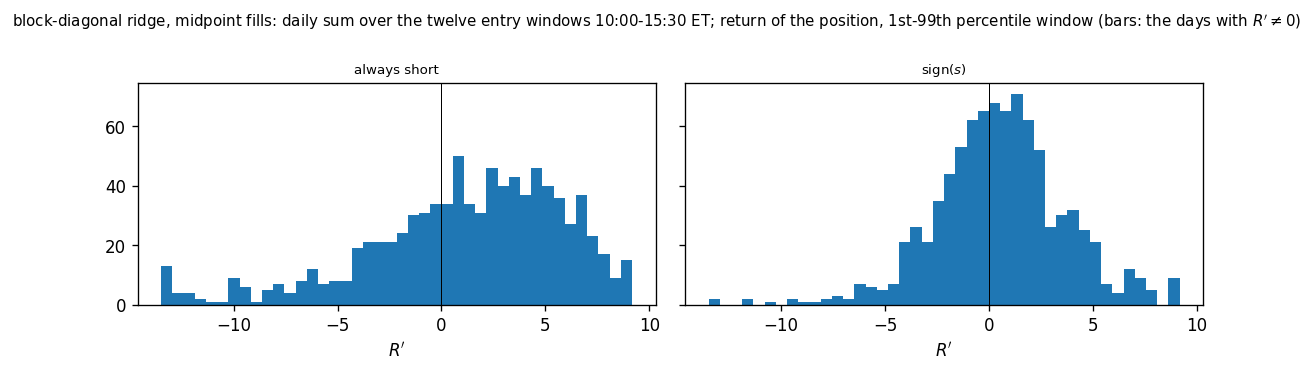
\includegraphics[width=0.45\textwidth]{../results/atm_straddle_intraday_holdclose/rule_by_strategy_dh/pooled/rule_hists_blk2_pooled.png}\par\smallskip
\small Distribution of the return of the daily sum over the twelve entry windows, block-diagonal ridge forecast, one panel per rule (returns inside their 1st--99th percentile window).
\end{center}
\begin{center}
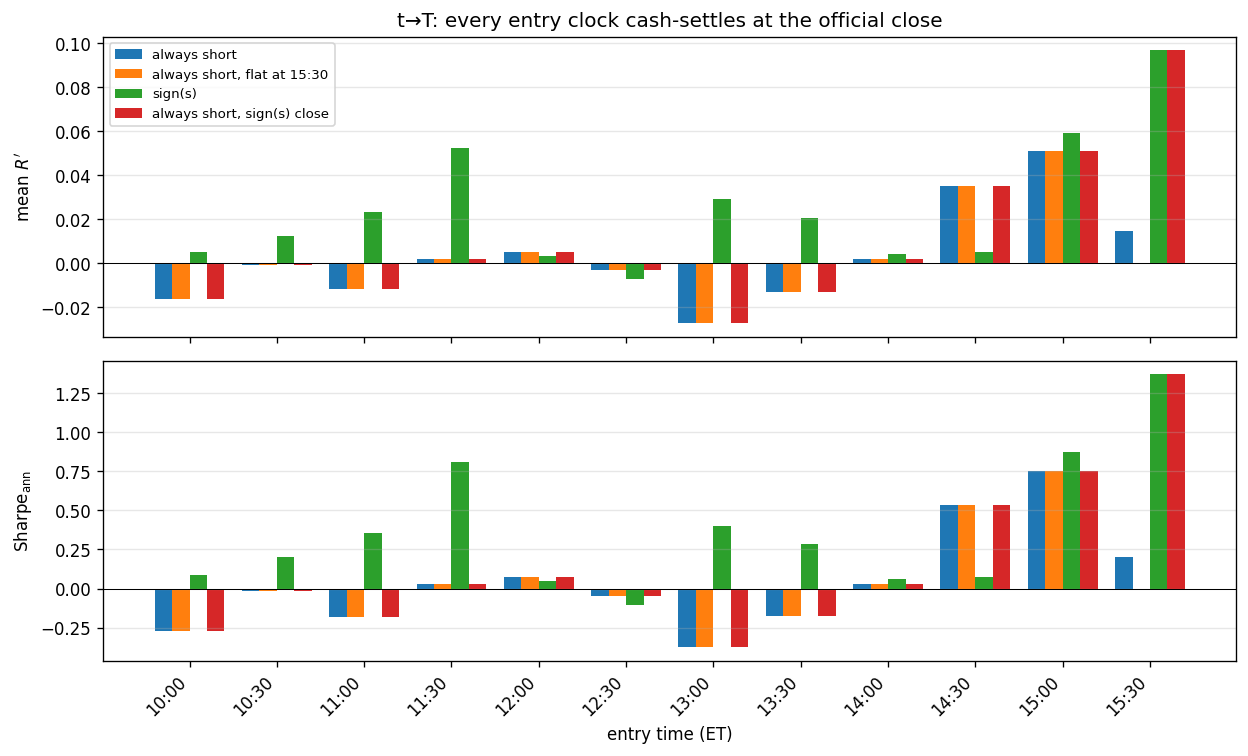
\includegraphics[width=0.45\textwidth]{../results/atm_straddle_intraday_holdclose/mean_by_entry_hhmm_as.png}\par\smallskip
\small Mean $R'$ and Sharpe$_{\mathrm{clk}}$ by entry clock (grouped bars). Sharpe$_{\mathrm{clk}}$ is that clock's daily series $\times\sqrt{252}$, not the pooled Sharpe$_{\mathrm{ann}}$. Delta-hedged $t\to T$: hold entry $K$ to official close, rebalance $\Delta$ every 30 minutes.
\end{center}
\begin{center}
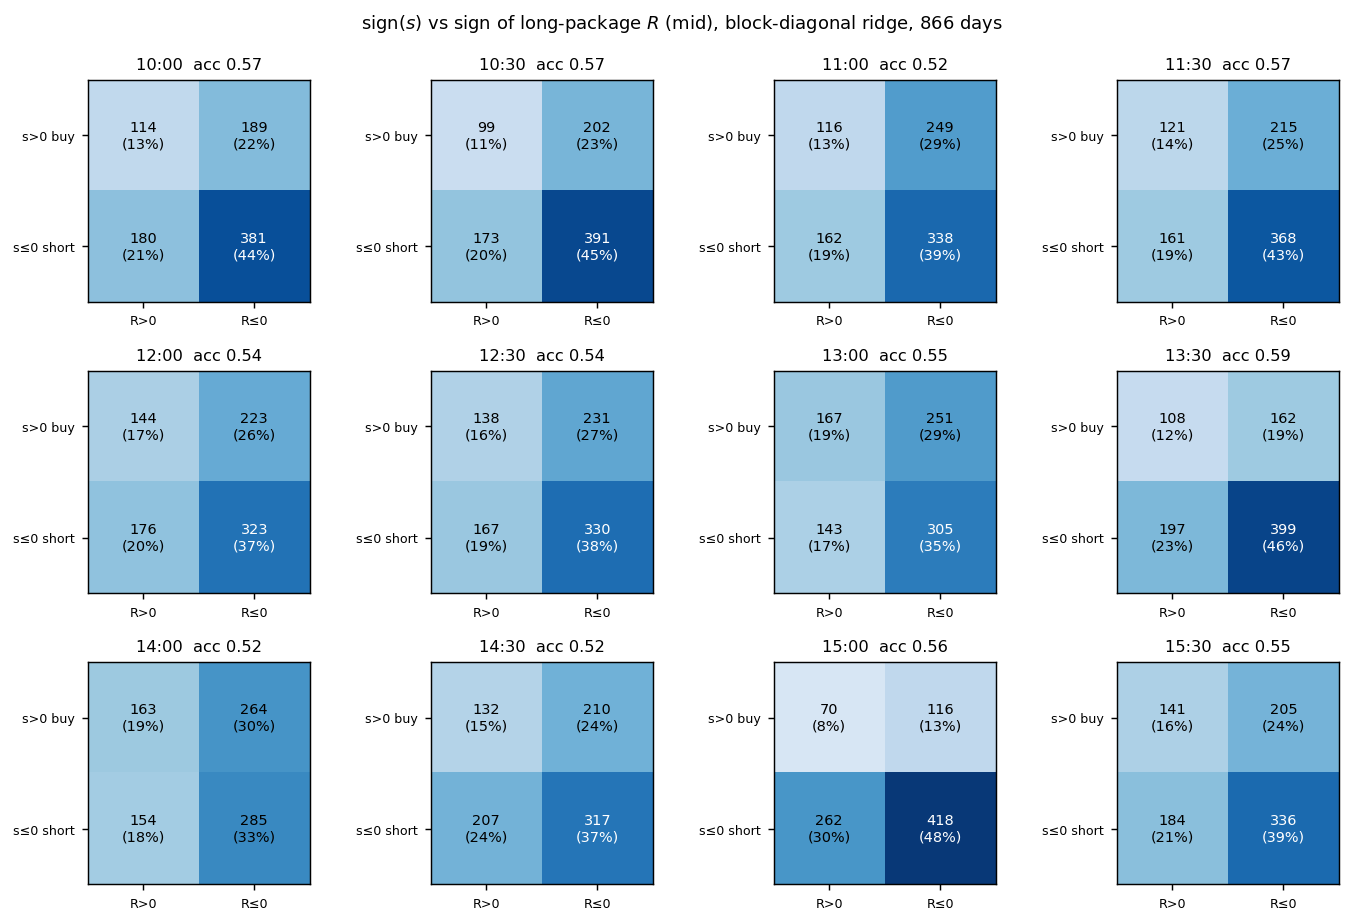
\includegraphics[width=0.45\textwidth]{../results/atm_straddle_intraday_holdclose/confusion_by_clock.png}\par\smallskip
\small Confusion matrix per entry clock: $\mathrm{sign}(s)$ (buy if $s>0$) against the sign of the long-package midpoint return. 15:30 is the paper trade.
\end{center}
\vspace{1ex}
\noindent\small Each row is the daily sum of the twelve overlapping remaining-session books: enter at each clock 10:00--15:30 ET, hold those strikes to the official close, delta-hedge every 30 minutes. 866 expiration days, 2020-01-03 to 2024-04-30 (the deck's frame). Fills are at the quoted midpoint everywhere except the last column, which is the same rule at the crossed spread: entry at the touch (the ask when long, the bid when short) and cash-settle at the official close (no exit spread).
\vspace{1ex}
\noindent\small One expiration day = one return; mid fill. Every $t$ here is the plain $t=\sqrt{n}\cdot\mathrm{mean}/\mathrm{std}$, with no autocorrelation correction. ``ex.\ kurt'' is the bias-corrected sample excess kurtosis (Gaussian $=0$). The short-volatility rule takes no forecast, so it is one row for all models. \textbf{Two Sharpes.} Both multiply by $\sqrt{252}$ because an expiration day is the unit of time (same year-length as the paper). They are not the same object. On a \emph{single-clock} page, Sharpe$_{\mathrm{clk}}=(\mathrm{mean}/\mathrm{std})\times\sqrt{252}$ of that clock's series: one remaining-session short per expiration day (enter at this clock, hold those strikes to the close, delta-hedge every 30 minutes). It answers ``if I only entered at this clock, what is my annual Sharpe?'' It is \emph{not} the book's Sharpe$_{\mathrm{ann}}$. On the \emph{pooled} page, Sharpe$_{\mathrm{ann}}=(\mathrm{mean}/\mathrm{std})\times\sqrt{252}$ of $R^{day}_d=\sum_t R'_{d,t}$, the sum of the day's twelve overlapping remaining-session books. That reserved name is the book's daily P\&L after pooling the session. The twelve books overlap; they are not twelve successive 30-minute holds. Sharpe$^{\times}$ is the same convention at the crossed spread. Every other column is daily. $n_{\mathrm{buy}}$ is the number of expiration days with position $>0$ (always-short is 0; on the pooled page it is days the sum of the twelve positions is positive); \%buy is $100\cdot n_{\mathrm{buy}}/n$, the notebook's column. The other column this table adds to the deck's is Sharpe$^{\times}_{\mathrm{ann}}$, the same rule's annualized Sharpe at the \emph{crossed spread} instead of the midpoint; every other column is the deck's.

\smallskip
\noindent\small Forecasts: baseline (HAR + calendar OLS); block-diagonal ridge (HAR block and exogenous block, separate penalties) on the design carrying the FOMC calendar block, and the same ridge on the earlier design without those columns, as a diagnostic row; LightGBM and XGBoost on the all-features design; lasso on the same design, causally tuned vs.\ fixed $\alpha=10^{-4}$; elastic net (causally tuned). $\dagger$ marks a column still fitted on the earlier design panel; a run of those four on the panel of record is pending. The signal is $s_t=\widehat{RV}_t-\mathrm{IV}^{2}_{\mathrm{hr}}h_t w_t$: the forecast against the implied variance of the same window. $w_t$ is the expanding mean of each prior day's remaining-session share of realized variance, $\mathrm{RV}_t/\sum_{s\ge t}\mathrm{RV}_s$ (in-fit panel history back to 2001), not the ratio of trailing clock-means. On the bars whose vendor implied volatility is a censored solver node the deck's treatment is used here too --- the volatility that reproduces the package midpoint, recovered by bisection over the remaining $h_t$ hours --- so every bar carries a signal and no bar sits flat.
\end{document}
